\section{Single Variable Quasi-Newton Methods}
%Single variable minimization and root finding are similar numerical exercises.
%Both activities are aimed at finding solutions to the equation $f(x) = 0$, although minimization may not necessarily solve such an equation.\footnote{In essence, root finding can be posed as a minimization problem, but the converse is not true}

The application of fundamental principles of modeling and mechanics often leads to an algebraic or transcendental equation that cannot be easily solved and represented in a closed form.  
In these cases a numerical method is required to obtain an estimate of the root or roots of the expression.  

Newton's method is an iterative technique that can produce good estimates of solutions to such equations.  
The method is employed by rewriting the equation in the form $f(x)=0$, then successively manipulating guesses for $x$ until the function evaluates to a value close enough to zero for the modeler to accept.
  
Figure \ref{fig:ArbitraryFunction} is a graph of some function whose intercept with the $x-$axis is unknown.  
The goal of Newton's method is to find this intersection (root) from a realistic first guess.  
Suppose the first guess is $x_1$, shown on the figure as the right-most specific value of $x$. 
The value of the function at this location is $f(x_1)$.  
Because $x_1$ is supposed to be a root the difference from the value zero represents an error in the estimate.  
Newton's method simply provides a recipe for corrections to this error.  

\begin{figure}[h!] %  figure placement: here, top, bottom, or page
   \centering
   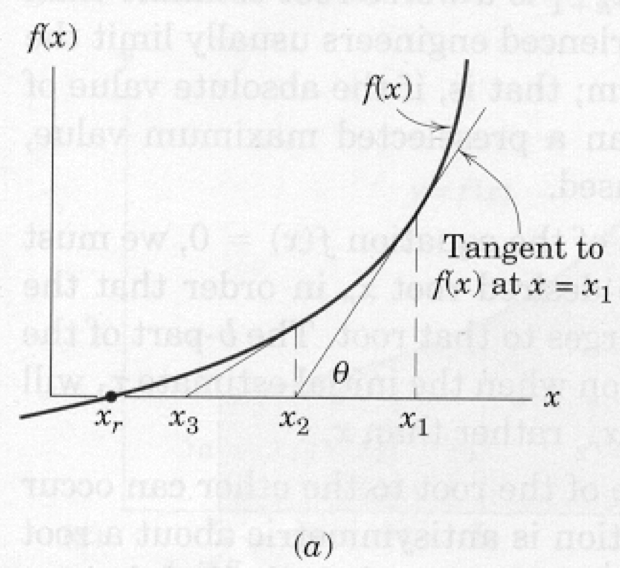
\includegraphics[width=4in]{./4-SVNewton/ArbitraryFunction.jpg} 
   \caption{Graph of Arbitrary Function.}
   \label{fig:ArbitraryFunction}
\end{figure}

Provided $x_1$ is not near a minimum or maximum (slope of the function is not zero) then a better estimate of the root can be obtained by extending a tangent line from $x_1,f(x_1)$ to the $x$-axis.  
The intersection of this line with the axis represents a better estimate of the root.

This new estimate is $x_2$.  
A formula for $x_2$ can be derived from the geometry of the triangle $x_2$,$f(x_1)$,$x_1$.   
Recall from calculus that the tangent to a function at a particular point is the first derivative of the function.  
Therefore, from the geometry of the triangle and the definition of tangent we can write,
\begin{equation}
tan(\theta)=\frac{df}{dx}\Biggr\vert_{x_1} = \frac{f(x_1)}{x_1 - x_2}
\end{equation}

Solving the equation for $x_2$ results in a formula that expresses $x_2$ in terms of the first guess plus a correction term.
\begin{equation}
x_2=x_1 - \frac{f(x_1)}{\frac{df}{dx}\vert_{x_1}} 
\end{equation}

The second term on the right hand side is the correction term to the estimate on the right hand side.  
Once $x_2$ is calculated we can repeat the formula substituting $x_2$ for $x_1$ and $x_3$ for $x_2$ in the formula.  
Repeated application usually leads to one of three outcomes:
\begin{enumerate}
\item a root;
\item divergence to $\pm\infty$; or 
\item cycling.
\end{enumerate}

These three outcomes are discussed below in various subsections along with some remedies.


The generalized formula is 

\begin{equation}
x_{k+1}=x_{k} - \frac{  f(x_{k})  }{   \frac{df}{dx}\rvert_{x_k} } 
\label{eqn:NewtonFormula}
\end{equation}

If the derivative is evaluated using analytical derivatives the method is called Newton's method, if approximations to the derivative are used, it is called a quasi-Newton method.

\subsection{Newton's Method --- Using analytical derivatives}
This subsection presents an example in \textbf{R} of implementing Newton's method with analytical derivatives.   
The algorithm itself is:
\begin{enumerate}
\item Write the function in proper form, and code it into a computer.
\item Write the derivative in proper form and code it into a computer.
\item Make an initial guess of the solution (0 and 1 are always convenient guesses).
\item Evaluate the function, evaluate the derivative, calculate their ratio.
\item Subtract the ratio from the current guess and save the result as the update.
\item Test for stopping:
\begin{enumerate}
\item Did the update stay the same value? Yes, then stop, probably have a solution.
\item Is the function nearly zero?  Yes, then stop we probably have a solution.
\item Have we tried too many updates? Yes, then stop the process is probably cycling, stop.
\end{enumerate}
\item If stopping is indicated proceed to next step, otherwise proceed back to step 4.
\item Stopping indicated, report last update as the result (or report failure to find solution), and related information about the status of the numerical method.
\end{enumerate}

The following example illustrates these step as well as a \textbf{R} implementation of Newton's method.

Suppose we wish to find a root (value of $x$) that satisfies Equation \ref{eqn:FindARoot}.
\begin{equation}
f(x) = e^x - 10 cos(x) -100
\label{eqn:FindARoot}
\end{equation}

Then we will need to code it into a script.   Here is a code fragment that will work:
\begin{lstlisting}[caption=R code fragment for the function calculation, label=lst:NewtonsFunction]
# Define Function Here
func <- function(x)
{
  func <- exp(x)-10*cos(x)-100;
  return(func);
}
\end{lstlisting}

%Notice in the code fragment we import three built-in functions from the \textbf{Python} \texttt{math} package, specifically $\exp()$, $\sin()$, and $\cos ()$.

The next step is to code the derivative.   In this case, Equation \ref{eqn:DerFind} is the derivative of Equation \ref{eqn:FindARoot}.

\begin{equation}
\frac{df}{dx}\vert{(x)} = e^x + 10 \sin(x)
\label{eqn:DerFind}
\end{equation}

A code fragment to compute the value of the derivative at any value of $x$ that will work is:

\begin{lstlisting}[caption=R code fragment for the derivative calculation, label=lst:NewtonsDerivative]
# Define Derivative Here
dfdx <- function(x)
{
  dfdx <- exp(x) + 10*sin(x); 
  return(dfdx);
}
\end{lstlisting}

Next we will need script to read in an initial guess, and ask us how many trials we will use to try to find a solution, as well as how close to zero we should be before we declare victory.   
\newpage

\begin{lstlisting}[caption=R code fragment for reading input data from the programmer, label=lst:InputNewtonData]
# Read some values from the console
message('Enter an initial guess for X for Newton method :  ')
xnow <- as.numeric(readline())
message('Enter iteration maximum :  ')
HowMany <- as.numeric(readline())
message('Enter a tolerance value for stopping (e.g. 1e-06) :  ')
HowSmall <- as.numeric(readline())
## There are several other ways to make these reads!  The scan() function would probably also work.
\end{lstlisting}



The use of \texttt{HowSmall}; is called a zero tolerance.   We will use the same numerical value for two tolerance tests.   Also notice how we are using error traps to force numeric input.   Probably overkill for this example, but we already wrote the code in an earlier chapter, so might as well use the code.  Professional codes do a lot of error checking before launching into the actual processing --- especially of the processing part is time consuming, its worth the time to check for obvious errors before running far a few hours then at some point failing because of an input value error that was predictable.

Now back to the tolerance tests. The first test is to determine if the update has changed or not.   If it has not, we may not have a correct answer, but there is no point continuing because the update is unlikely to move further.   The test is something like

\begin{math}
\text{IF}~\lvert x_{k+1} - x_{k} \rvert < \text{Tol.~ THEN Exit and Report Results}
\end{math}  

The second test is if the function value is close to zero.   The structure of the test is similar, just an different argument.   The second test is something like

\begin{math}
\text{IF}~\lvert f(x_{k+1}) \rvert < \text{Tol.~ THEN Exit and Report Results}
\end{math} 

One can see from the nature of the two tests that a programmer might want to make the tolerance values different.   This modification is left as a reader exercise.

Checking for maximum iterations is relatively easy, we just include code that checks for normal exit the loop.\footnote{Rather than breaking from the loop.}

Now we simply connect the three fragments, and we have a working \textbf{R} script that implements Newton's method for Equation \ref{eqn:FindARoot}.  
Listing \ref{lst:NewtonsMethod} is the entire code module that implements the method, makes the various tests, and reports results.
Figure \ref{fig:NewtonTrials} is a screen capture of the program run in \textbf{R}.

The example is specific to the particular function provided, but the programmer could move the two functions \texttt{func} and \texttt{dfdx} into a user specified module, and then load that module in the program to make it even more generic.   The next section will use such an approach to illustrate the ability to build a generalized Newton method and only have to program the function itself.

\newpage
\begin{lstlisting}[caption=R code demonstrating Newton's Method calculations, label=lst:NewtonsMethod]
# Newtons Method in R
# Define Function Here
func <- function(x)
{
  func <- exp(x)-10*cos(x)-100;
  return(func);
}
# Define Derivative Here
dfdx <- function(x)
{
  dfdx <- exp(x) + 10*sin(x); 
  return(dfdx);
}
# Newton's Method Here
# Read some values from the console
message('Enter an initial guess for X for Newton method :  ')
xnow <- as.numeric(readline())
message('Enter iteration maximum :  ')
HowMany <- as.numeric(readline())
message('Enter a tolerance value for stopping (e.g. 1e-06) :  ')
HowSmall <- as.numeric(readline())
# Now start the iterations
for (i in 1:HowMany) {
  xnew <- xnow - func(xnow)/dfdx(xnow)
# test for stopping
  if (abs(xnew-xnow) < HowSmall){
    message('Update not changing')
    xnow <- xnew
    print(cbind(xnow,xnew,func(xnew)))
    break
  }
  if (abs(func(xnew) < HowSmall)) {
    message('Function value close to zero')
    xnow <- xnew
    print(cbind(xnow,xnew,func(xnew)))
    break    
  }
# next iteration
xnow <- xnew
}
if (i >= HowMany){
  message('Iteration limit reached')
  print(cbind(xnow,xnew,func(xnew)))
}
\end{lstlisting}

\begin{figure}[h!] %  figure placement: here, top, bottom, or page
   \centering
   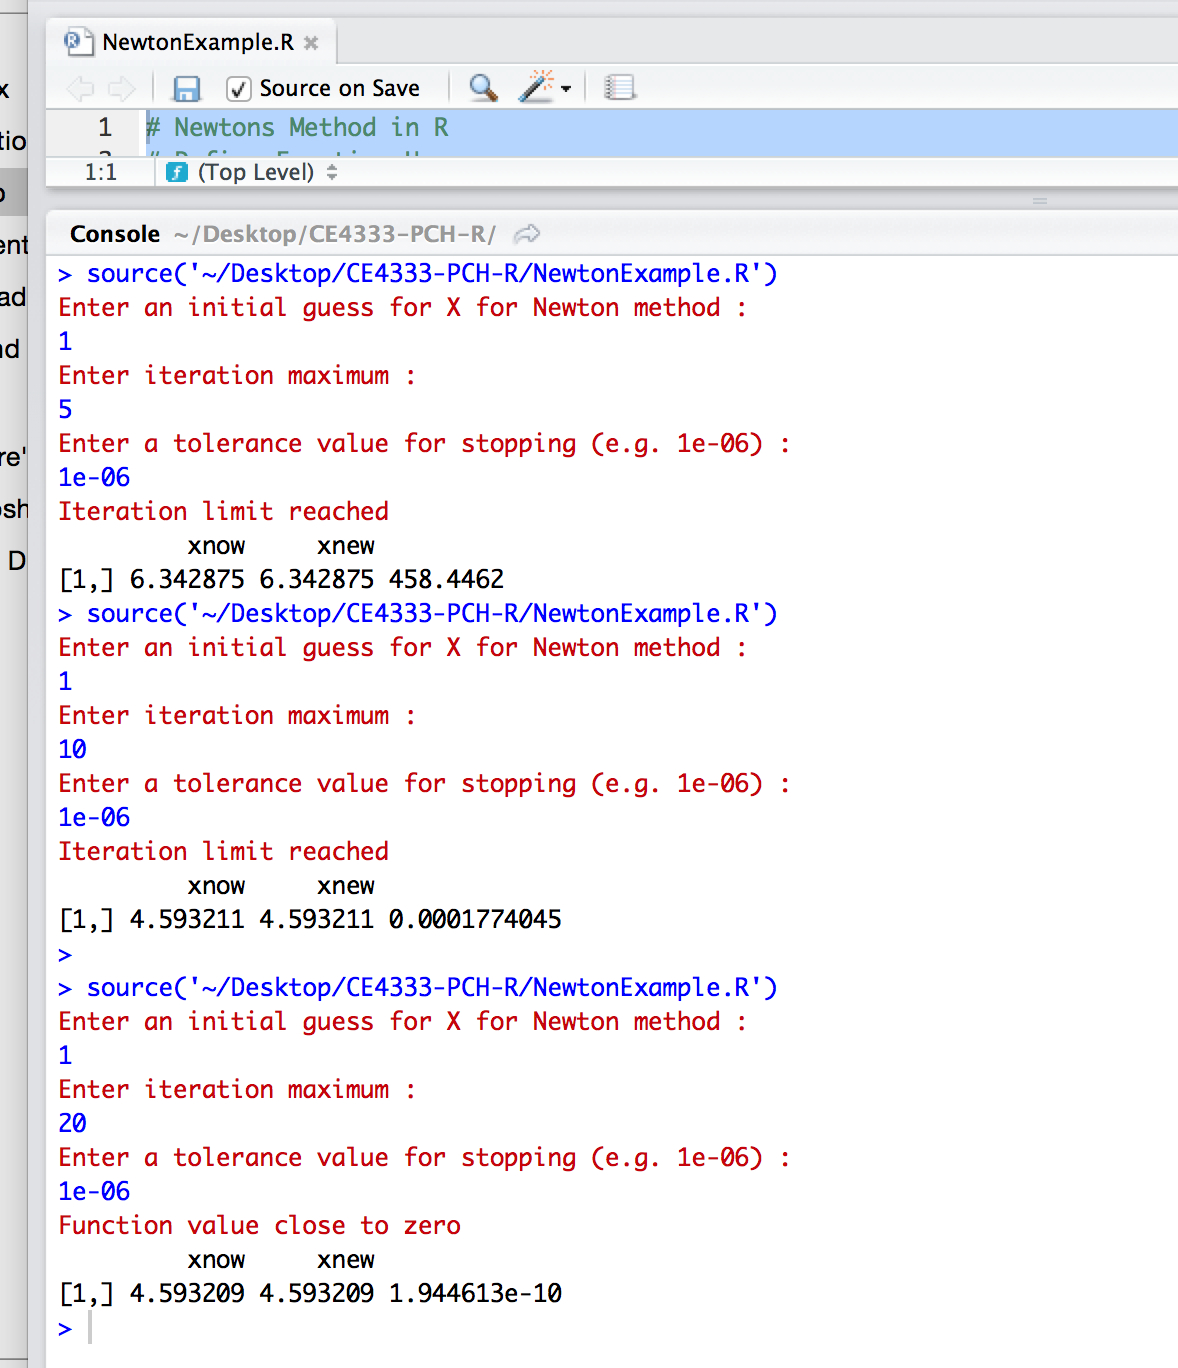
\includegraphics[width=6in]{./4-SVNewton/NewtonTrials.jpg} 
   \caption{Several runs of the program using the analytical derivative to illustrate different kinds of responses.}
   \label{fig:NewtonTrials}
\end{figure}

%%%%%%%%%%%%%%%%%%%%%%%%%%%%%%%%%%%%%%%%
\subsection{Newton's Method --- Using finite-differences to estimate derivatives}
A practical difficulty in using Newton's method is determining the value of the derivative in cases where differentiation is difficult.  
In these cases we can replace the derivative by a difference equation and then proceed as in Newton's method. 

Recall from calculus that the derivative was defined as the limit of the difference quotient:
\begin{equation}
\frac{df}{dx}\vert_{x} = \lim_{\Delta x \rightarrow 0}\frac{f(x + \Delta x) - f(x) }{\Delta x}
\end{equation}

A good approximation to the derivative should be possible by using this formula with a small, but non-zero value for $\Delta x$.

\begin{equation}
\frac{df}{dx}\vert_{x} \approx \frac{f(x + \Delta x) - f(x) }{\Delta x}
\end{equation}

When one replaces the derivative with the difference formula the root finding method the resulting update formula is

\begin{equation}
x_{k+1}=x_k - \frac{f(x_k) \Delta x}{f(x_k + \Delta x)-f(x_k)} 
\label{eqn:QuasiNewtonFormula}
\end{equation}

This root-finding method is called a quasi-Newton method.

Listing \ref{lst:QNewton}  is the code fragment that we change by commenting out the analytical derivative and replacing it with a first-order finite difference approximation of the derivative.  
The numerical value $1e-06$ is called the step size ($\Delta x$)  and should be an input value (rather than built-in to the code as shown here) like the tolerance test values, and be passed to the function as another argument.

\begin{lstlisting}[caption=R code demonstrating Newton's Method calculations, label=lst:QNewton]
# Define Derivative Here
dfdx <- function(x)
{
#  dfdx <- exp(x) + 10*sin(x); 
    dfdx <- (func(x + 1e-06) - func(x) )/ (1e-06);
# func must already exist before first call!
  return(dfdx);
}
\end{lstlisting}

Starting with the last example lets modify the analytical version of the code by inserting the above fragment in place of the analytical derivative.  Listing \ref{lst:QuasiNewton} is the listing with the modification in place.  Notice we have only changed a single line, and not have a more flexible tool.  The next modification (left as an exercise) is to detach the creation of the function from the main algorithm, then we would have a general purpose Quasi-Newton's method.

\begin{lstlisting}[caption=R code demonstrating Newton's Method calculations using finite-difference approximation for the derivative, label=lst:QuasiNewton]
# Newtons Method in R
# Define Function Here
func <- function(x)
{
  func <- exp(x)-10*cos(x)-100;
  return(func);
}
# Define Derivative Here
dfdx <- function(x)
{
#  dfdx <- exp(x) + 10*sin(x); 
  dfdx <- (func(x + 1.0e-06) - func(x))/(1.0e-06)
  return(dfdx);
}
# Newton's Method Here
# Read some values from the console
message('Enter an initial guess for X for Newton method :  ')
xnow <- as.numeric(readline())
message('Enter iteration maximum :  ')
HowMany <- as.numeric(readline())
message('Enter a tolerance value for stopping (e.g. 1e-06) :  ')
HowSmall <- as.numeric(readline())
# Now start the iterations
for (i in 1:HowMany) {
  xnew <- xnow - func(xnow)/dfdx(xnow)
# test for stopping
  if (abs(xnew-xnow) < HowSmall){
    message('Update not changing')
    xnow <- xnew
    print(cbind(xnow,xnew,func(xnew)))
    break
  }
  if (abs(func(xnew) < HowSmall)) {
    message('Function value close to zero')
    xnow <- xnew
    print(cbind(xnow,xnew,func(xnew)))
    break    
  }
# next iteration
xnow <- xnew
}
if (i >= HowMany){
  message('Iteration limit reached')
  print(cbind(xnow,xnew,func(xnew)))
}
\end{lstlisting}



Listing \ref{lst:QuasiNewton} is the main code.  Notice how the function definitions are changed, in particular \texttt{dfdx}.



Figure \ref{fig:NewtonTrials2} is a screen capture of the program run after the code modification above.   
\begin{figure}[h!] %  figure placement: here, top, bottom, or page
   \centering
   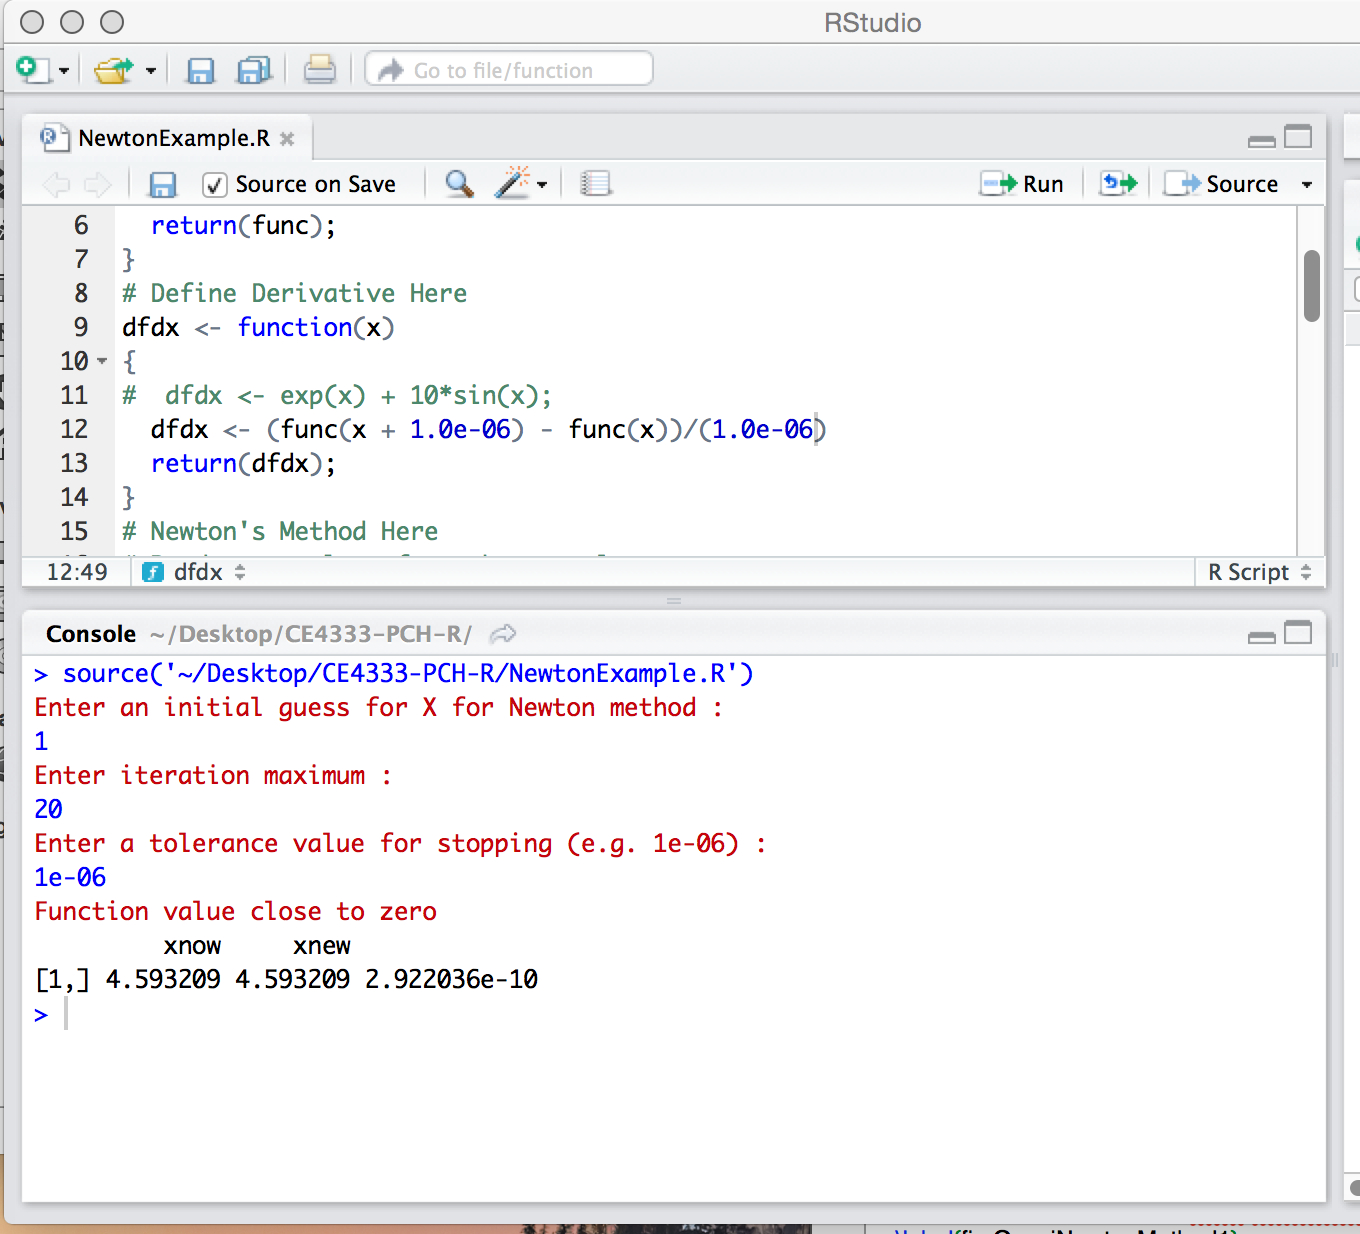
\includegraphics[width=6in]{./4-SVNewton/NewtonTrials2.jpg} 
   \caption{Program run after changing from analytical to finite-difference approximation for the derivative.}
   \label{fig:NewtonTrials2}
\end{figure}

The~advantage of the approximate derivative is that we don't have to do the calculus --- just code in the function.  

The obvious advantage of modular coding is to protect the parts of the code that are static, and just modify the function definitions.   We can keep a working example around in case we break something and use that to find what we broke.

\subsection{Method Fails}
The three subsections below describe the ways that the method routinely fails, along with some suggestions for remedy.   Generally we should plot the function before trying to find a root, but sometimes the root finding is a component of a more complex program and we just want it to work.   In that situation, the programmer would build in many more tests that the three above to try to force a result before giving up.   
\subsubsection{Multiple Roots}
Figure \ref{fig:MultipleRoots} illustrates the behavior in the presence of multiple roots.  
When there are multiple roots the method will converge on the root that that is defined by the initial guess.\footnote{This behavior is called ``sensitive dependence on initial conditions''.}  
The initial estimate must be close enough to the desired root to converge to the root.\footnote{Ironically, we need a good idea of the answer before we start the method.}
\begin{figure}[h!] %  figure placement: here, top, bottom, or page
   \centering
   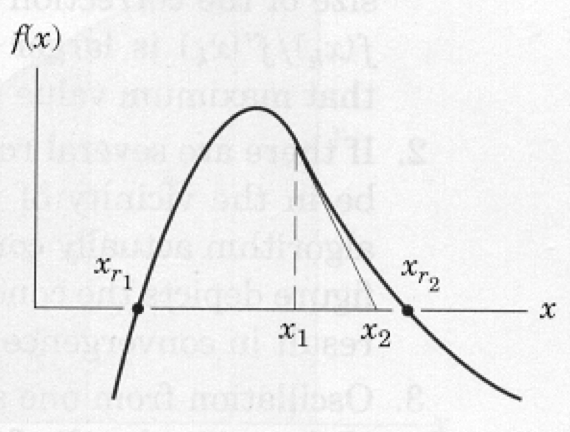
\includegraphics[width=4in]{./4-SVNewton/MultipleRoots.jpg} 
   \caption{Multiple roots.}
   \label{fig:MultipleRoots}
\end{figure}
Another challenge is what happens if the initial guess is at the divide (the peak of the function in Figure \ref{fig:MultipleRoots}); in such cases we may actually get a divergent solution because the slope of the function at that peak is nearly zero.  
\subsubsection{Cycling}
Cycling can occur when the root is close to an inflection point of the function.  
Usual practice is to again limit the step size to prevent such behavior.  
Figure \ref{fig:RootCycling} is an illustration of cycling.
\begin{figure}[h!] %  figure placement: here, top, bottom, or page
   \centering
   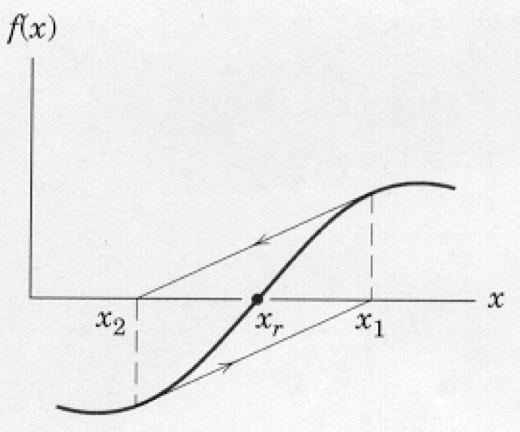
\includegraphics[width=4in]{./4-SVNewton/RootCycling.jpg} 
   \caption{Estimates cycling around a root.}
   \label{fig:RootCycling}
\end{figure}
A good remedy for cycling is to first detect the cycling, then provide a small ``shove'' to the guess.  
Examination of root finding codes often reveals a pseudo-random number generator within the code that will provide this shove when cycling is detected.
\subsubsection{Near-zero derivatives}
The derivative in Equation \ref{eqn:NewtonFormula} must not be zero, otherwise the guess corresponds to a maximum or minimum of the function and the tangent line will never intersect the x-axis.    
The derivative must not be too close to zero, otherwise the slope will be so small as to make the correction too large to produce a meaningful update.  Usual practice is to limit the size of the correction term to some maximum and to use this maximum value whenever the formula prescribes a larger step.
Divergence to $\pm\infty$ is usually explained by near-zero derivatives at the sign change. 
The bi-section method is a little more robust in this respect.
\subsection{Related Concepts}
A couple of other root finding methods are worth mentioning because they can sometimes serve as a fallback when Newton's method fails.   Two robust methods are bisection and false-positioning.
\subsubsection{Root finding by bisection}
\subsubsection{Root finding by false-positioning}


\subsection{Exercises}
\begin{enumerate}
\item Build a Newton's Method program (or use mine) and make the program request a tolerance value for ``how close to zero'' is the function, and ``how small is the change in update values.''  Build your code using the modular approach (two files).  Test your code using the same example in the notes.

\item Now modify the main and the function module to use approximate derivatives (the finite-difference formulation) and require the user supply a step size.   Test the code using the same example in the notes.

For each of the exercises above, prepare documentation similar to the notes where you describe the salient points of your program.   

\item  Now use your program to find roots for the following equations:
\begin{enumerate}
\item $\exp(x) - 3x^2 =0$ \\
\item $\ln(x) - x + 2 = 0$ \\
\item $\tan(x) - x - 1 = 0$ \\
\end{enumerate}
For these three equations, document your search for roots.  Identify if there are bad initial guesses that cause the program to fail to find a root.   Also the equations may have multiple roots.  If you discover multiple roots, identify the starting values one needs to use to converge to a particular root.


\end{enumerate}

%%%%%%%%%%%%%%%%%%%%%%%%%%%%%%%%%%%%%%%%%%%%%%%%%%%%%%%%%%%%%
%%%%%%%%%%%%%%%%%%%%%%%%%%%%%%%%%%%%%%%%%%%%%%%%%%%%%%%%%%%%%%
\clearpage



